\documentclass[11pt]{article}

\usepackage{amsmath,amssymb,graphicx}
\usepackage[margin=1in]{geometry}
\usepackage{booktabs}
\usepackage{array}
\usepackage{hyperref}

% Alternative restrained titles:
% Phase-Corridor-Controlled Texture Transition in a Clustered DK Branch
% Reduction and One-Sided Closure of a Clustered DK Interaction Sector

\title{Effective Smeared-Transfer Closure in a Clustered DK Sector}
\author{Tomislav Rupi\'c \\ Independent Researcher}
\date{March 2026}

\begin{document}

\maketitle

\begin{abstract}
A clustered Dirac--K\"ahler interaction sector on the frozen HAOS (Harmonic Address Operating System) / IIP (Interaction Invariance Physics) branch was tested under mechanism non-generality, reduced-model extraction, phase-closure, and mechanism-isolation passes. The braid-like signature did not generalize beyond clustered seeds and therefore fails as a family-wide intrinsic mechanism. Nevertheless, the clustered braid/smear sector admitted a valid two-state effective reduction and a one-sided closed phase diagram whose stable connected region lies in a smeared-dominant regime. Mechanism isolation identified the phase corridor as the primary control variable for the local braid/smear split, with geometry overlap and $0 \leftrightarrow 1$ operator cross-coupling acting as secondary supports, while grade transfer did not emerge as the primary driver on the frozen branch. On this branch, braid-like exchange is therefore retained only as a clustered texture-level descriptor, not as a stable closed phase or universal mechanism.
\end{abstract}

\section{Scope and Branch Discipline}

This paper concerns only the frozen clustered Dirac--K\"ahler branch of Phase III in the HAOS-IIP pre-geometry atlas program. The result is branch-bounded and clustered-sector bounded throughout. It does not establish a family-wide intrinsic braid mechanism, does not support a stable braid phase, and does not promote clustered braid texture into a universal topological ontology. The paper is therefore about the actual closed content of one frozen branch, not about a general braid law for the broader program.

The operative discipline is negative-boundary preservation. Every positive statement below remains compatible with the exclusions frozen in Stages 23.10 through 23.14. Local effective validity in the clustered sector is kept distinct from family-wide generality, and descriptive braid texture is kept distinct from stable closed mechanism.

\section{Frozen Setup and Implementation Constraints}

The branch uses the frozen clustered Dirac--K\"ahler collision sector on a regular lattice with static Gaussian kernel class, fixed interaction update, fixed timestep policy, and no memory, selector logic, or adaptive kernel terms. Later Phase III work perturbs only within that frozen discipline: clustered seed geometry, relative phase placement, bounded graded-support surrogates where a literal degree-spectrum change is unavailable on the regular lattice, and bounded local weakening of selected operator couplings.

Several implementation constraints matter for interpretation. The effective reduction stage uses the resolved $3 \times 3$ anchor lattice in phase and bounded clustered-seed detuning rather than a broader exploratory mesh. The phase-closure stage treats weak coupling $\beta \in \{0.01, 0.02\}$ as an internal stability probe inside the $5 \times 3$ phase-width grid rather than as an external expansion of the primary lattice. The mechanism-isolation stage uses bounded blockwise grade-fraction anchoring as a grade-transfer suppression surrogate because the frozen branch does not expose a literal transfer-off switch without changing operator class. These are implementation constraints of the frozen branch, not hidden strengths.

\section{Non-Generality of Braid Across Families}

The decisive negative result of Stage 23.10 is that braid-like exchange does not generalize beyond clustered seeds. The family-comparison probe returned robust non-clustered braid hits $= 0$, raw non-clustered braid hits $= 0$, clustered braid hits $= 2$, and clustered degraded collapse $= \mathrm{True}$. The clustered baseline remained braid-like, but mild clustered degradation moved to transfer-smeared, and all six non-clustered comparison families remained non-braid.

That combination fixes the first boundary of Phase III. The braid read is not a family-wide intrinsic mechanism of the frozen Dirac--K\"ahler branch. At most it is a clustered texture artefact with limited clustered robustness. Any later interpretation must therefore begin from clustered-sector restriction rather than from an intrinsic braid premise.

\begin{figure}[t]
\centering
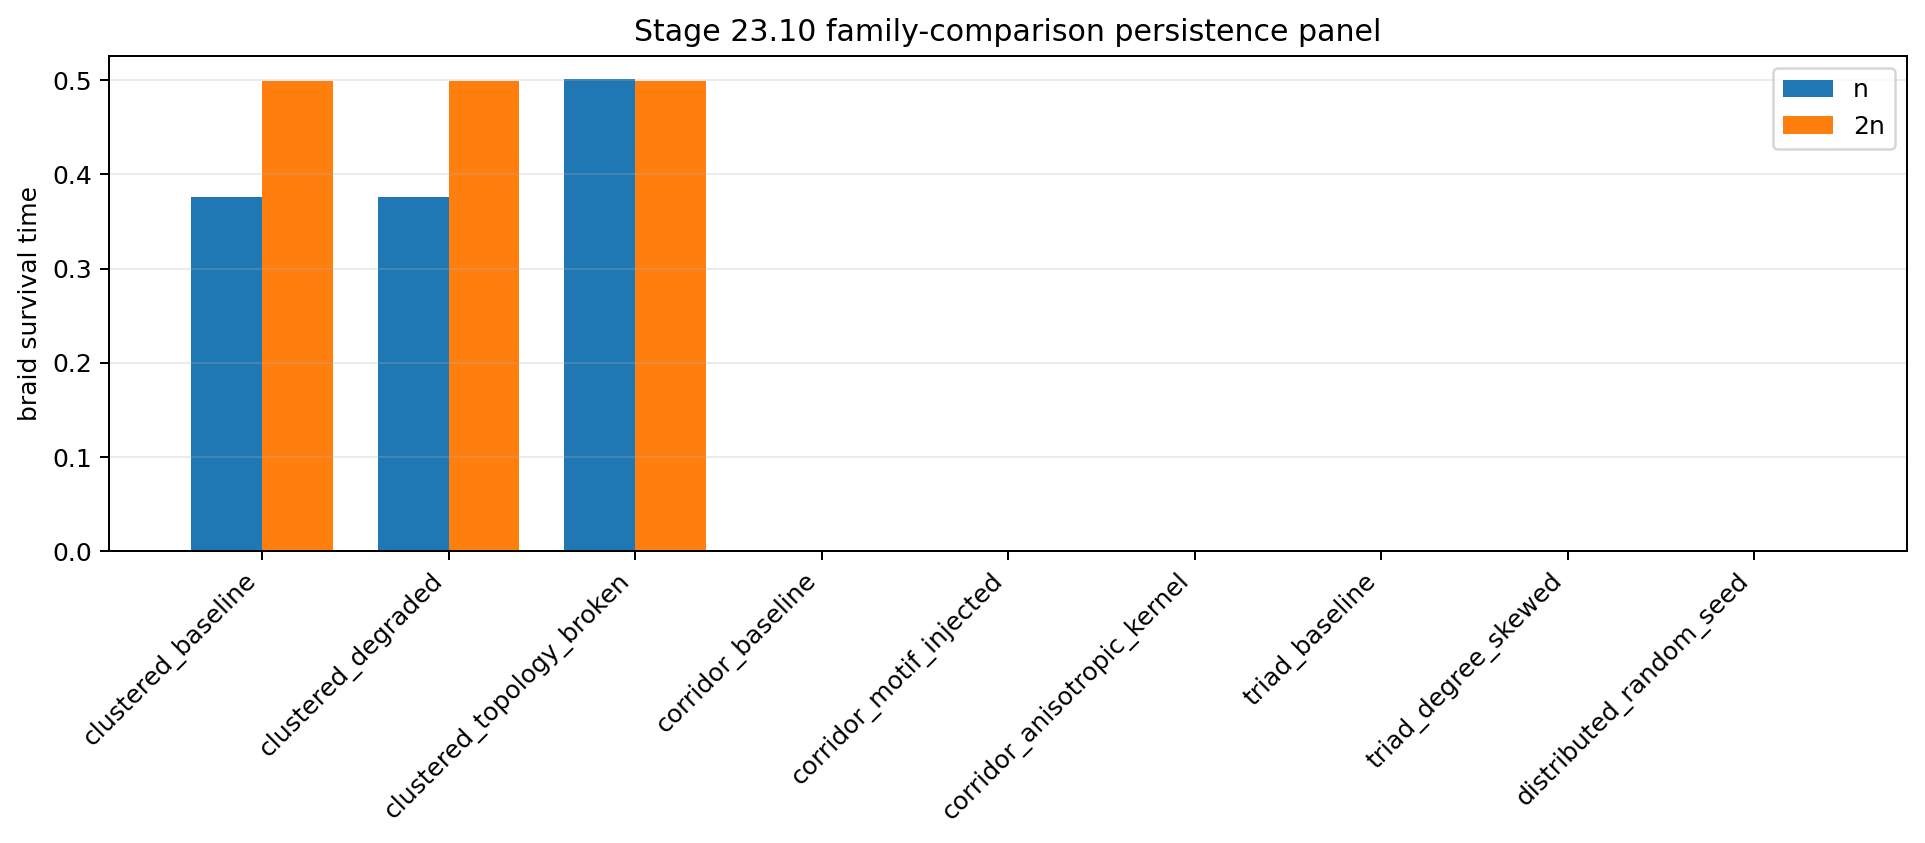
\includegraphics[width=0.92\linewidth]{../plots/20260316_102709_stage23_10_family_comparison_persistence_panel.png}
\caption{Stage 23.10 family-comparison summary. The braid label remains confined to clustered seeds and does not reappear in the six non-clustered comparison families.}
\label{fig:family_non_generality}
\end{figure}

\section{Minimal Effective Reduction in the Clustered Sector}

Once the family-wide claim failed, the remaining question became whether the surviving clustered braid/smear texture admitted a compact effective description. Stage 23.11 answered that question positively on the tested anchor lattice. The reduction pass returned \texttt{effective\_model\_valid = TRUE} with topology agreement $= 1.0000$, detuning threshold error $= 0.0000$, phase-band width error $= 0.0000$, and mean survival-time envelope mismatch $= 0.0139$.

This validates a two-state effective surrogate for the clustered braid/smear sector under the tested reduction pass. The result is narrow but real: the clustered sector can be compressed into a valid low-dimensional descriptive model without reopening the family-wide braid question. The reduction therefore survives, but only as a clustered texture surrogate. It does not overturn the non-generality result and does not elevate the braid read beyond its clustered scope.

\section{Effective Phase Diagram Closure}

Stage 23.12 then asked whether the clustered sector admits a closed effective phase description once refinement, weak-coupling consistency, and reverse evolution are enforced together. The answer is positive but one-sided. The closure pass returned \texttt{phase\_diagram\_closed = TRUE} with \texttt{closure\_class = smeared\_dominant\_closed\_phase\_diagram}. The only refinement-/beta-/reverse-stable connected region is the strong-asymmetry row \texttt{width\_ratio = 1.35}, and it remains stable across the sampled phase corridor $0.375 \rightarrow 0.575$.

The same closure pass freezes the second major negative boundary: no stable braid phase survives, and no localized encounter phase survives. Symmetric and moderate-asymmetry cells remain transient mixed under the tested closure pass. The clustered DK sector therefore closes as a finite smeared-transfer effective regime, but the closure is explicitly one-sided. The surviving closed content is on the smeared side, not on the braid side.

\begin{figure}[t]
\centering
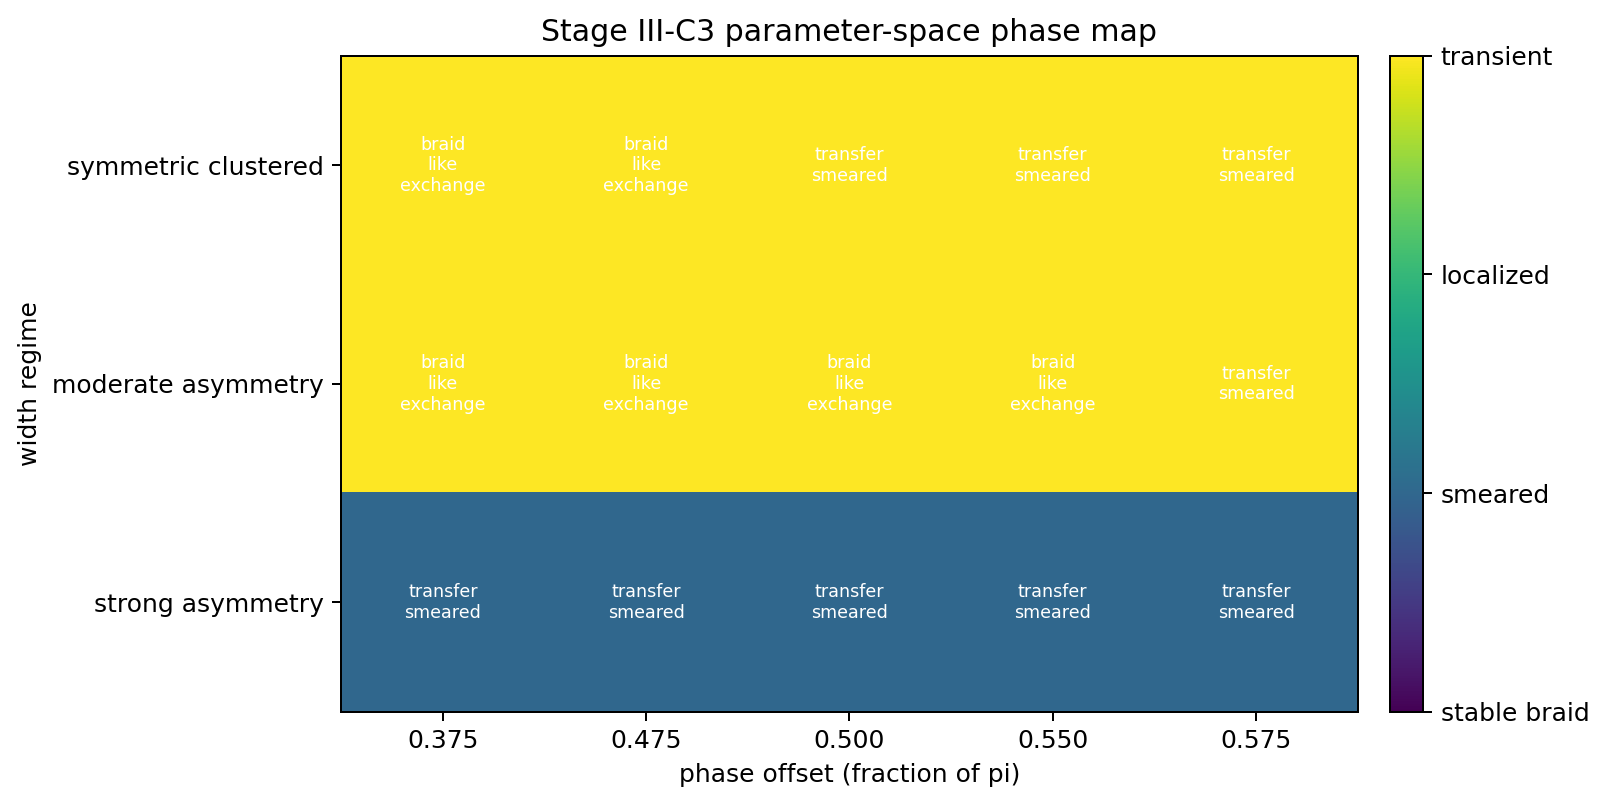
\includegraphics[width=0.88\linewidth]{../plots/20260316_105448_stage23_12_effective_phase_map.png}
\caption{Stage 23.12 effective phase map. The closed connected region is one-sided and smeared-dominant; no stable braid phase survives the closure pass.}
\label{fig:phase_closure}
\end{figure}

\section{Mechanism Isolation}

Stage 23.13 isolates what actually controls the local braid/smear split inside the clustered sector. The mechanism read closes as \texttt{phase\_corridor\_primary}. Weak and moderate phase flattening both move the clustered control from braid-like exchange to transfer-smeared while remaining in a bounded dynamical regime. Geometry-overlap weakening and $0 \leftrightarrow 1$ operator cross-coupling suppression act only as secondary supports: each kills the braid read only at moderate ablation, not at weak ablation. Grade transfer does not emerge as the primary driver on the frozen branch.

The mechanism sentence of Phase III is therefore narrower than any earlier braid-centered reading. The clustered braid/smear split is primarily phase-corridor controlled, with geometry overlap and $0 \leftrightarrow 1$ operator cross-coupling acting as bounded secondary supports. This explains the local texture transition without upgrading it into a universal braid mechanism.

\begin{figure}[t]
\centering
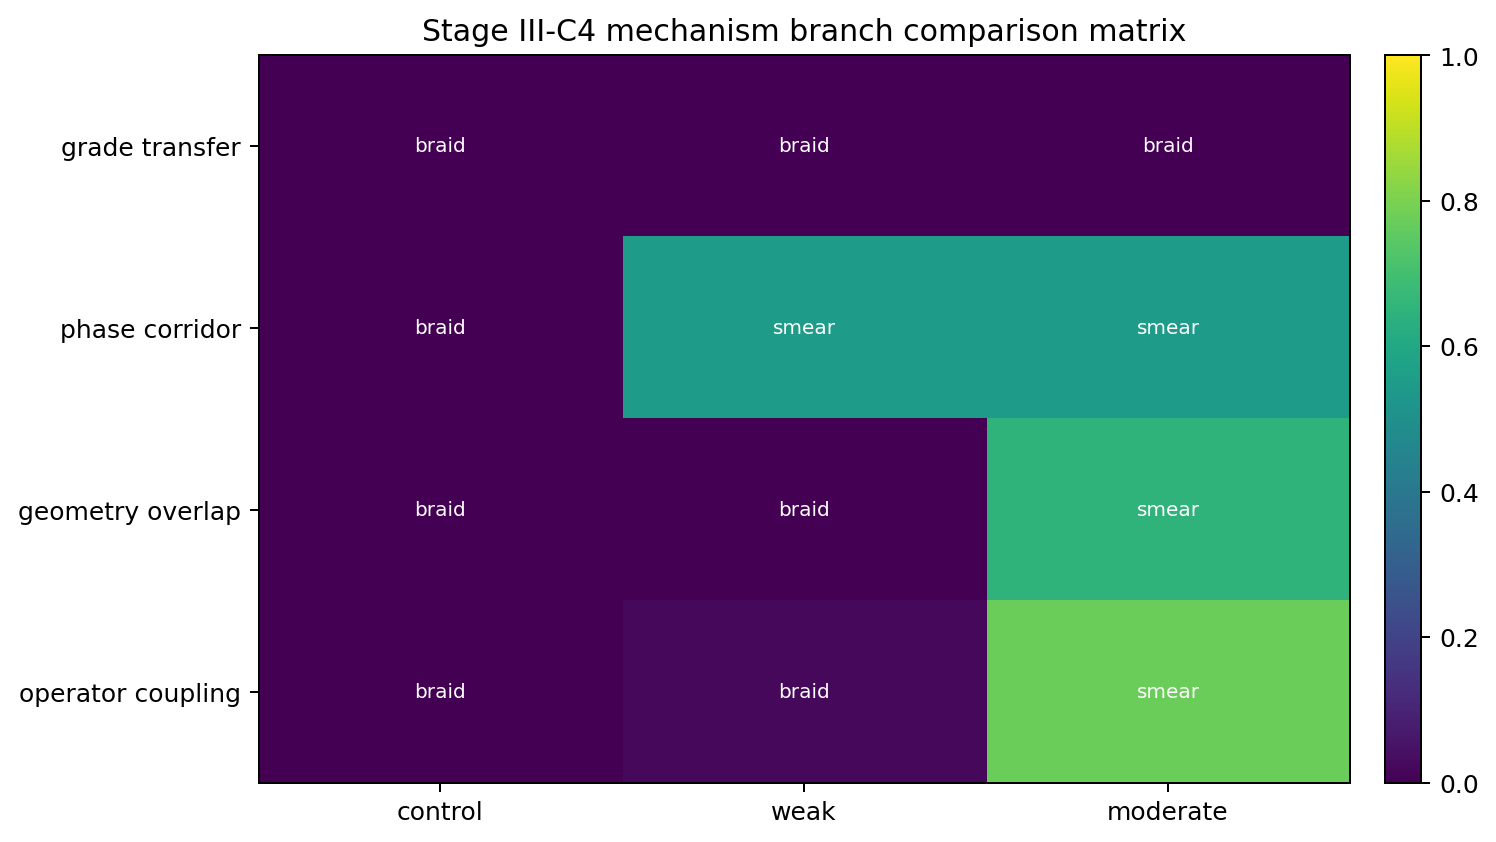
\includegraphics[width=0.90\linewidth]{../plots/20260316_110320_stage23_13_mechanism_branch_comparison_matrix.png}
\caption{Stage 23.13 mechanism-isolation summary. Phase flattening collapses the braid signal cleanly, while geometry-overlap weakening and operator cross-coupling suppression act only as secondary supports.}
\label{fig:mechanism_isolation}
\end{figure}

\section{Final Phase III Claim Ledger}

\begin{table}[t]
\centering
\small
\begin{tabular}{@{}p{1.1in}p{4.9in}@{}}
\toprule
Status & Claim \\
\midrule
Survives & The clustered DK braid/smear sector admits a valid two-state effective surrogate on the tested anchor lattice. \\
Survives & The clustered sector closes as a one-sided smeared-dominant closed phase diagram. \\
Survives & The only stable connected region is the explicit strong-asymmetry row \texttt{width\_ratio = 1.35} across the sampled phase corridor. \\
Survives & The controlling mechanism classification for the local braid/smear split is \texttt{phase\_corridor\_primary}. \\
Bounded support & Geometry overlap and $0 \leftrightarrow 1$ operator cross-coupling act only as secondary supports. \\
Fails & A family-wide intrinsic braid mechanism does not survive the family-comparison pass. \\
Fails & No stable braid phase survives the closure pass. \\
Fails & No localized encounter phase survives the closure pass. \\
Fails & Grade transfer is not the primary control variable on the frozen branch. \\
Excluded & The clustered braid-like texture may not be universalized into a topological law or ontology. \\
\bottomrule
\end{tabular}
\caption{Frozen Phase III claim ledger consolidated from Stages 23.10 through 23.14.}
\label{tab:claim_ledger}
\end{table}

The true content of the clustered DK branch is sharper than a simple braid narrative. Phase III separates texture from mechanism and mechanism from closure. The braid signature remains descriptively useful because it marks a local organized texture transition inside the clustered sector, but it is not structurally sovereign: it does not generalize across families, does not survive as a stable closed phase, and does not control the surviving effective closure. What closes is the smeared-transfer sector, and what controls the braid/smear split locally is the phase corridor.

\section{Discussion}

That is the mature reading of the branch. The local braid texture is neither denied nor inflated. It remains part of the phenomenology map, but only as a clustered descriptor whose appearance is subordinate to phase-corridor control and bounded by the negative closures established upstream. The positive core is therefore not ``a braid mechanism'' but a clustered-sector effective reduction plus one-sided smeared closure.

\begin{figure}[t]
\centering
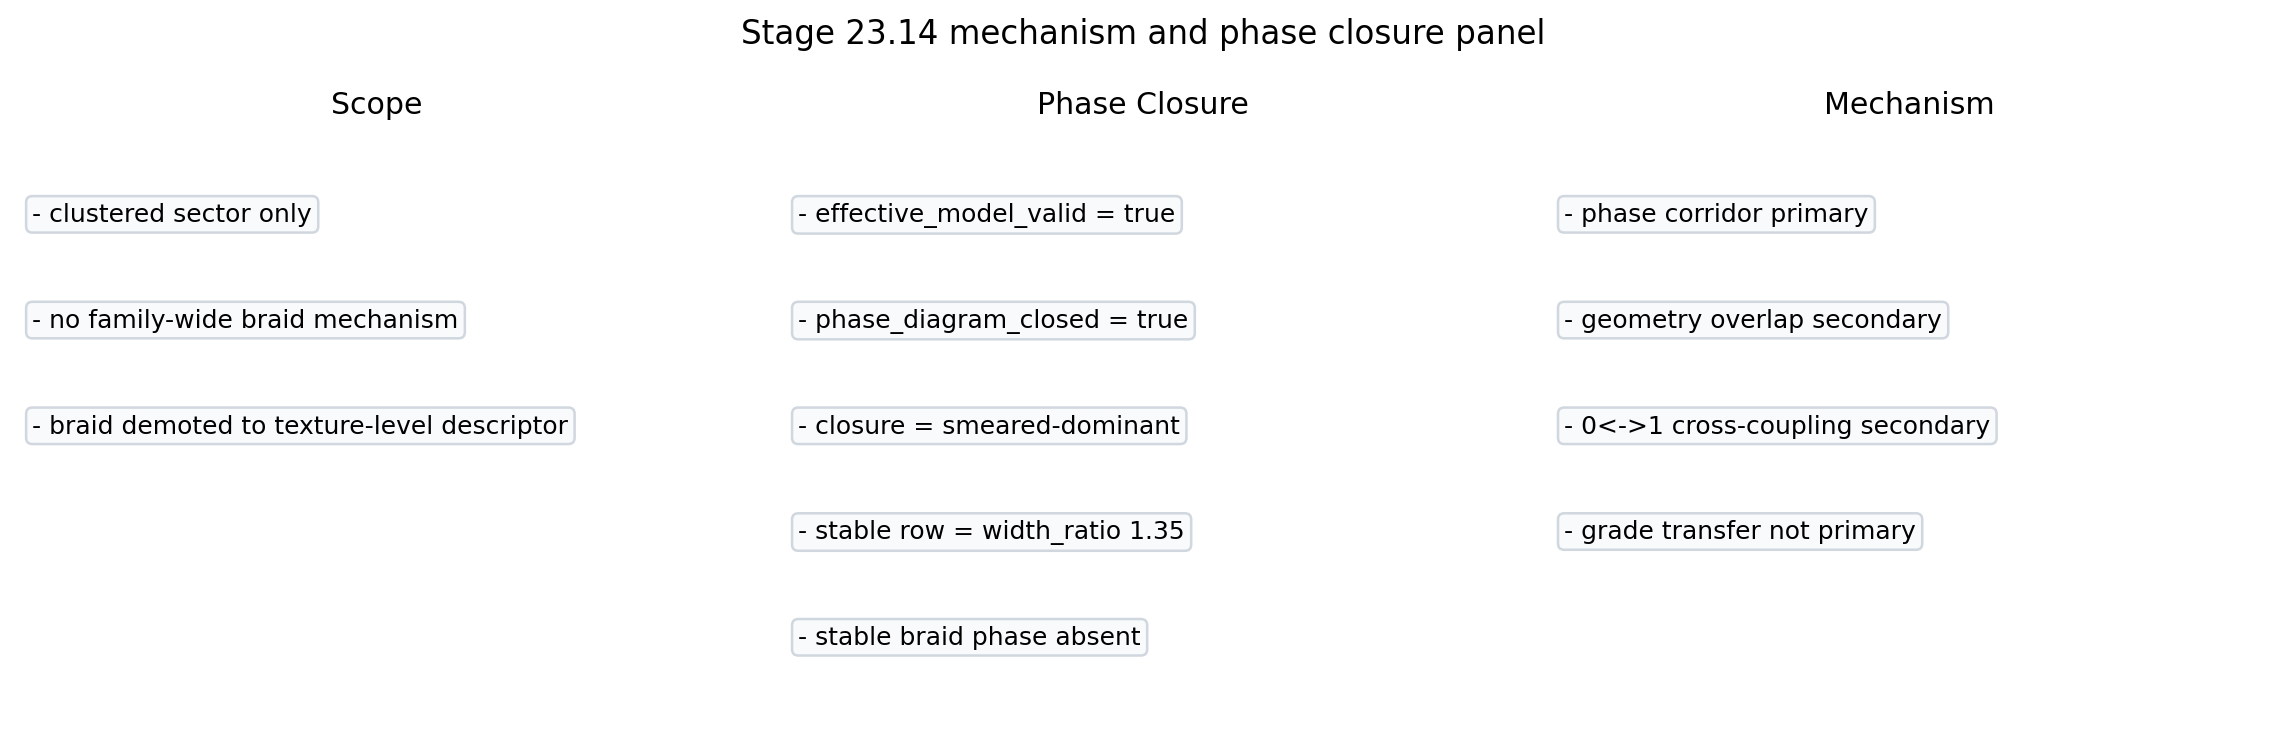
\includegraphics[width=0.92\linewidth]{../plots/20260316_111201_stage23_14_phaseIII_mechanism_and_phase_closure_panel.png}
\caption{Stage 23.14 consolidation panel. The positive core is a clustered-sector smeared-transfer closure with a phase-corridor-primary texture split, bounded by explicit negative claims.}
\label{fig:freeze_panel}
\end{figure}

\section{Restricted Correspondence to Standard Physics}

The present Phase III result is not a derivation of any standard continuum theory. Its connection to standard physics is narrower and branch-bounded. On the frozen clustered DK branch, a local texture transition admits a valid reduced effective description, closes into a one-sided smeared-dominant phase diagram, and is governed primarily by a phase-controlled mechanism with geometry overlap and $0 \leftrightarrow 1$ operator cross-coupling as bounded secondary supports. In that restricted sense, the branch aligns with standard physics practice at the level of effective regime description, mechanism isolation, and strict regime dependence.

No stronger identification is licensed here. On this branch alone, no equivalence to Maxwell, Dirac, gauge, or spacetime dynamics has been established; no conserved-quantity correspondence or observable dictionary has been derived; and the clustered braid-like signal remains a texture-level descriptor rather than a universal physical law. The non-generality result is part of this discipline: a phenomenon that appears only in the clustered sector and fails across families must be treated as sector-specific, not as a universal invariant.

\section{Limits of Interpretation}

The scope is strictly branch-bounded. Every claim in this paper is confined to the frozen clustered DK sector under the tested closure pass. There is no demonstrated portability to non-clustered families, no evidence for a stable braid phase, no evidence for a localized encounter phase, and no claim beyond the frozen operator class and its bounded surrogates. The paper therefore does not license a family-wide braid mechanism, a universal topological mechanism, or any broader ontological reading of the clustered braid texture.

Reopening the braid question now requires an explicit new branch with changed structural premises. Acceptable reopening moves would need to alter operator class, family regime, or another declared structural prior. Re-describing the same frozen branch in broader language would not count as new evidence.

\section{Conclusion}

Phase III on the frozen clustered DK branch resolves into a narrow but coherent closure. The family-wide braid claim fails, but a clustered-sector two-state effective reduction survives, and the closed phase content remains one-sided on the smeared side. Mechanism isolation then fixes the local control variable of the braid/smear split as the phase corridor, with geometry overlap and $0 \leftrightarrow 1$ operator cross-coupling acting only as secondary supports.

Any relation to standard physics remains, on this branch, restricted to effective-structure correspondence rather than established continuum equivalence. On the frozen clustered DK branch, the surviving Phase III content is a finite smeared-transfer effective sector with a phase-corridor-controlled braid/smear split, while braid-like exchange itself remains a clustered texture descriptor rather than a family-wide intrinsic mechanism.

\end{document}
